\documentclass[../main.tex]{subfiles}
\begin{document}

\section{Preliminary Measurements and Settings}

\subsection{Planes Characterisation}
\label{subsec:planecalibration}
\noindent In order to perform the experiment, it is mandatory to find optimal working points for the PMTs coupled to the scintillator planes. The variables to optimise are the voltage and the threshold at which the two PMTs in each plane work: the former influencing the gain while the latter moderates dark current effects introduced by high working voltage. The 3B group performed the calibration of the P3 plane, its PMTs being 03 and 04. Calibration of 01, 02, 11, 12 PMTs were performed by the 1B and 2B groups, respectively.\\

The characterisation is performed with the following procedure. A logical AND of the 2 PMTs in the reference plane (P1) is implemented. This output is then connected separately with each one of the PMTs of the plane to characterise. The registered counts obtained with this procedure are called Coincidence Counts. Also counts directly out of each PMT were registered, these being called Single Counts. For each voltage and threshold the setup registers counts for a fixed time of 100\,s and the counts (both Single PMT-A,B and Coincidence PMT-A,B) are registered. For each sweep across any configuration a working plateau-like region is expected for the coincidence counts.\\

In order to realise the circuit described in the previous paragraph the signal of the PMTs, digitised by the LED which also controls the threshold of the signals, is sent into a CAEN N455 Quad Coincidence Logic Unit producing the 3 required ANDs. Furthermore, to obtain the counts, the signals are sent to a CAEN N1145 Quad Scaler. This unit has a clock that can be used to consistently measure how many events are registered in standard time windows. The unit presents 4 displays, showing the counts in each one of the 4 channels, namely the single PMT-A,B and their AND coincidence with the reference plane. Finally, via the GECO software it is possible to perform a scan of the powering voltages. During this scan the reference plane is set at \SI{1000}{\volt} with a \SI{40}{\milli \volt} threshold. After the voltage scan, the threshold scan is performed modifying the threshold of the signals in the LED unit. In this case the reference plane is set to \SI{1000}{\volt} with a \SI{2}{\milli \volt} threshold in order to achieve maximum sensitivity during the scan.\\

The results of the scans for coincidence counts of the 3 planes are shown in Figure \ref{fig:hvthr}, where the uncertainties are given by the resolution of the threshold in the LED unit while on poissonian counts the associated uncertainty is the square root of the counts themselves. From the observed behaviours, the settings of all the planes were decided to be at a tension of \SI{1050}{\volt} with LED threshold at \SI{30}{\milli \volt}. These settings, despite being apparently allowed by the scans, resulted in some difficulties which are addressed in Section \ref{sec:res}.

\begin{figure}[htb!]
    \centering
    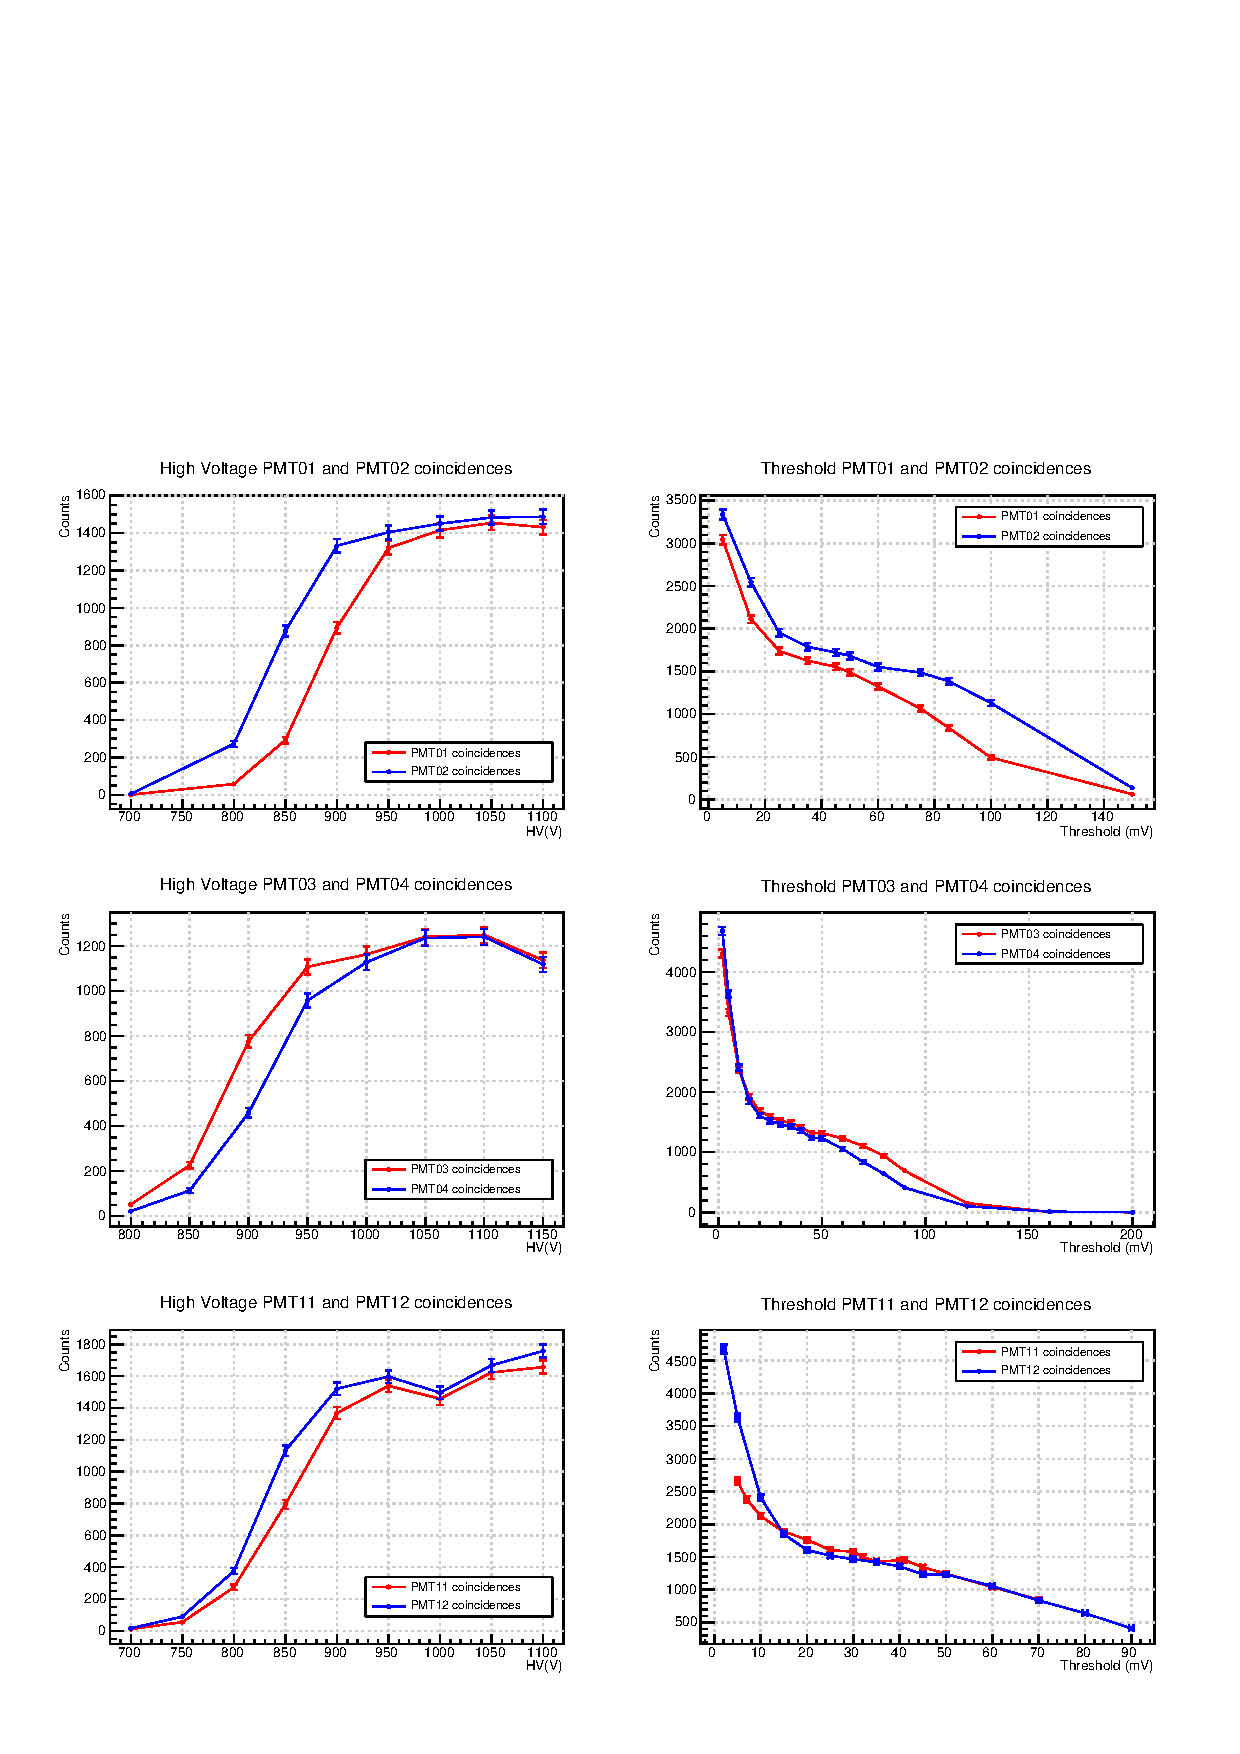
\includegraphics[width = \linewidth]{images/hv-thr.pdf}
    \caption[High Voltage and Threshold scans for scintillating planes]{High Voltage and Threshold scans for scintillating planes. From these behaviours working points have been decided to be at \SI{1050}{\volt} for high voltage and \SI{30}{\milli \volt} for threshold.}
    \label{fig:hvthr}
\end{figure}

\subsection{Background and Efficiency Measurements} \label{subsec:bkg}
Another important step of the calibration is the proper estimation of expected background, since in some cases it can lead to wrong results, if not treated correctly.

An estimate of the background can be obtained constructing a circuit such that the trigger is given by the CAEN N93B Dual Timer module. As such, the trigger window gets opened by the dual timer module and not by the proper passing of a real muon. In this way stop signals will be randomly collected from stops in the planes not related to a decay in the absorber, thus creating the shape of the expected background. Unfortunately, due to time constraints the setup did not have enough time to collect a sample large enough for the proper estimation of the expected background, also in part due to the choice of a low acquisition rate dictated by the technical limitations of the PC acquiring the data. On the other hand, the background behaviour can be estimated from the collected data leaving it as a free parameter in the final fit.

Moreover, an efficiency measurement has been performed for the three planes, despite it not having applications in the remaining of the experiment. To perform the efficiency measurement of a plane, the plane under analysis would be stacked between the other two planes. The digitised signals of the top and bottom planes, taken as reference, get combined into a logic AND. Another logic AND gets realised using the output of all three planes. Using the counts given by the CAEN N1145 Quad Coincidence Unit it was possible to obtain an estimate of the efficiency of the planes above 95\% for each one of them. Efficiency measurements are shown in Table \ref{tab:efficiencies}.

\subsection{Time Scale Calibration}
The objective of the experiment is getting a time measurement of the lifetime of the muon. The experimental setup expresses time counts as clock cycles, which require proper treatment in order to be compared with standard time units. In order to do this one PMT signal from P1 and P2 have been substituted with fake signals generated with the CAEN N93B Dual Timer which should emulate a valid trigger from a passing muon in P1, P2 and finally stopping in the absorber, between P2 and P3, starting the clock. After the first counter, a second one is initiated, emulating an electron passing shortly after in all 3 planes, substituting the signal of the 2 remaining PMTs in P1 and P2 and one from P3, finally stopping the counter. The veto has been left untouched from the background measurement rack configuration, while the AND gates between PMT signals have been switched to OR gates. 

As in the previous paragraph, due to technical limitations in the acquisition rate of the PC, muon signals have been set at a rate of 10\,Hz. Furthermore, due to the Dual Timer module not being correctly calibrated, the times between the fake muon trigger and the fake electron stop have been separately measured using the oscilloscope, which provides on its own an uncertainty on the measure. The uncertainty on the measured number of clock cycles has been taken as the standard deviation between $\approx$1000 measures for each measured stopping time value. Calibration results are shown in Figure \ref{fig:timeCalibration}, which shows a complete agreement between the time measures for all 3 channels, leading to a conversion factor of 3.98(0)\,ns per clock cycle.

\begin{figure}[htb!]%
 \centering
 \subfloat[]{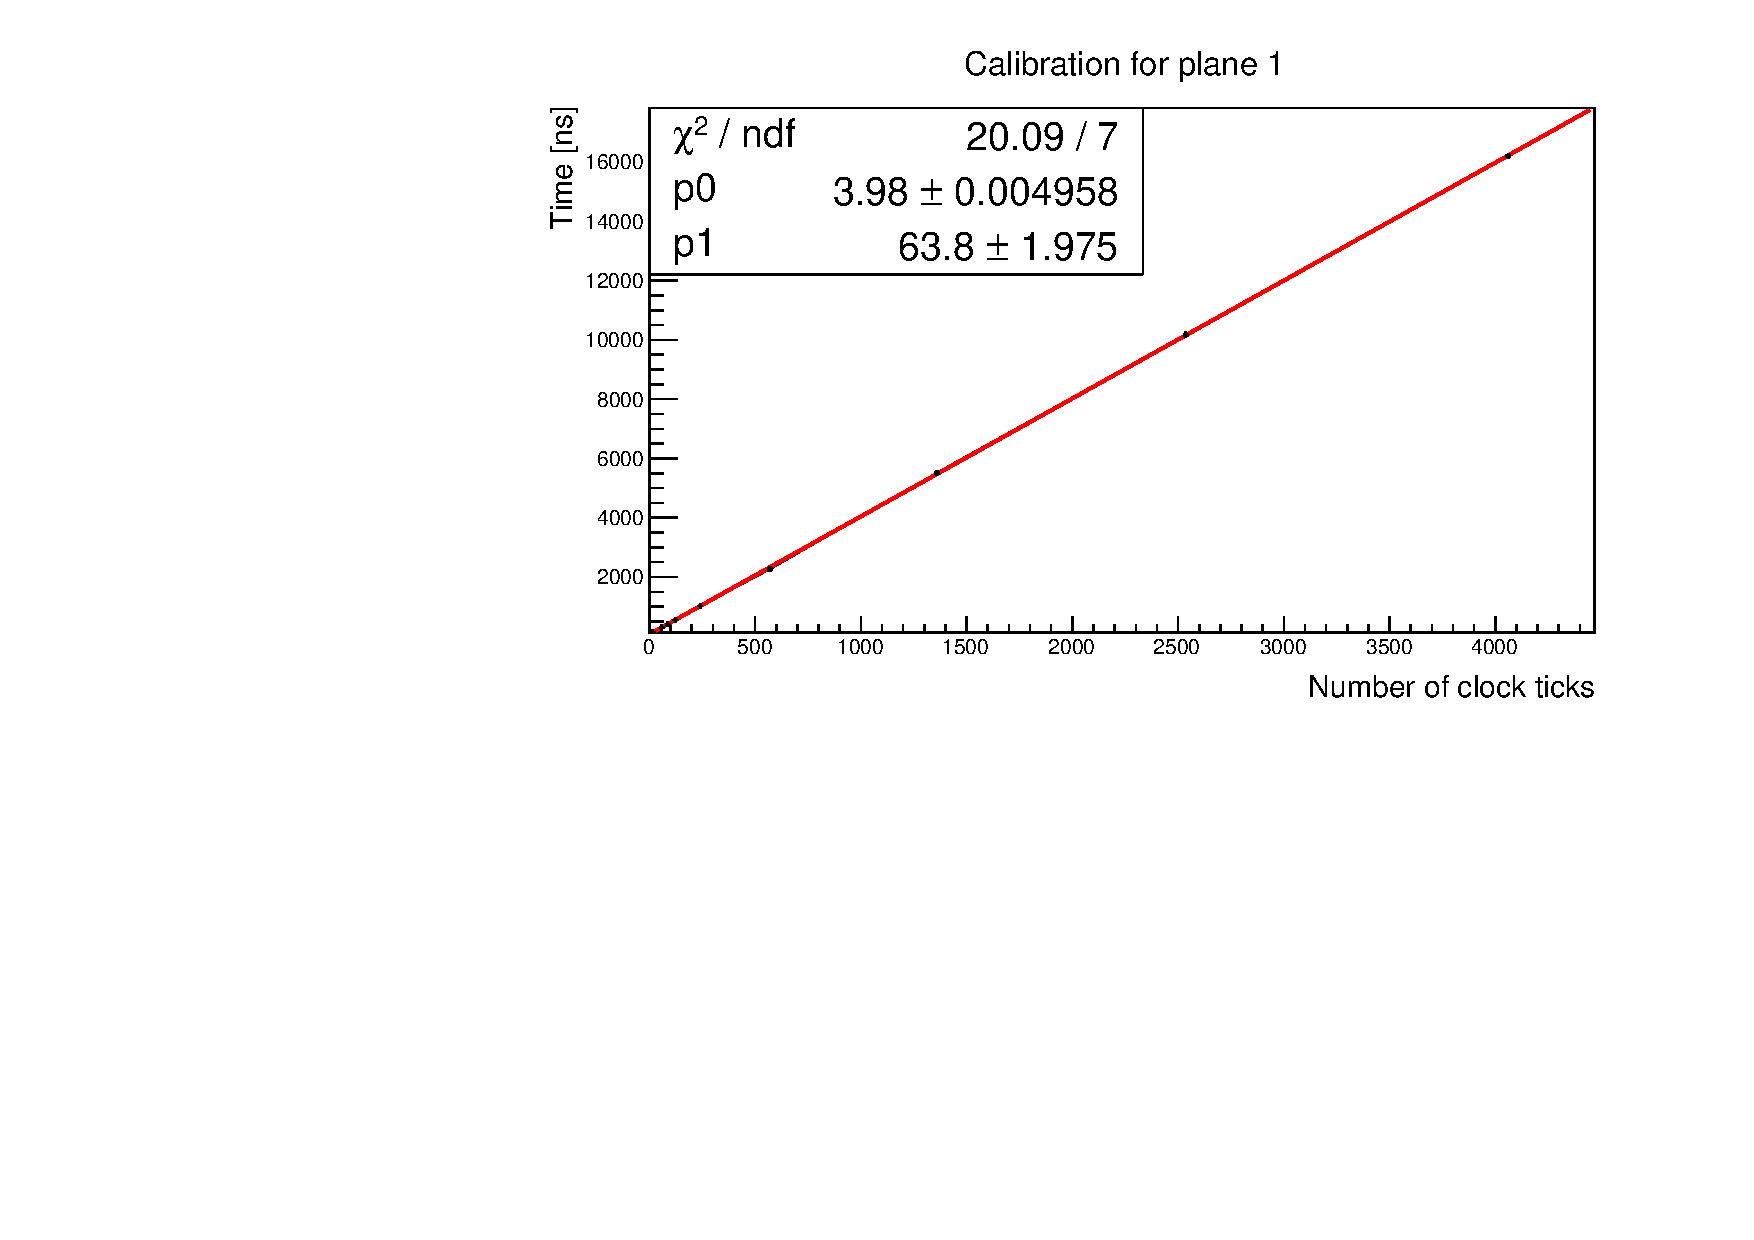
\includegraphics[width=0.7\linewidth]{images/calib_plane_1.pdf}}\\%{images/calib_plane_1.pdf}\label{fig:a}}
 \subfloat[]{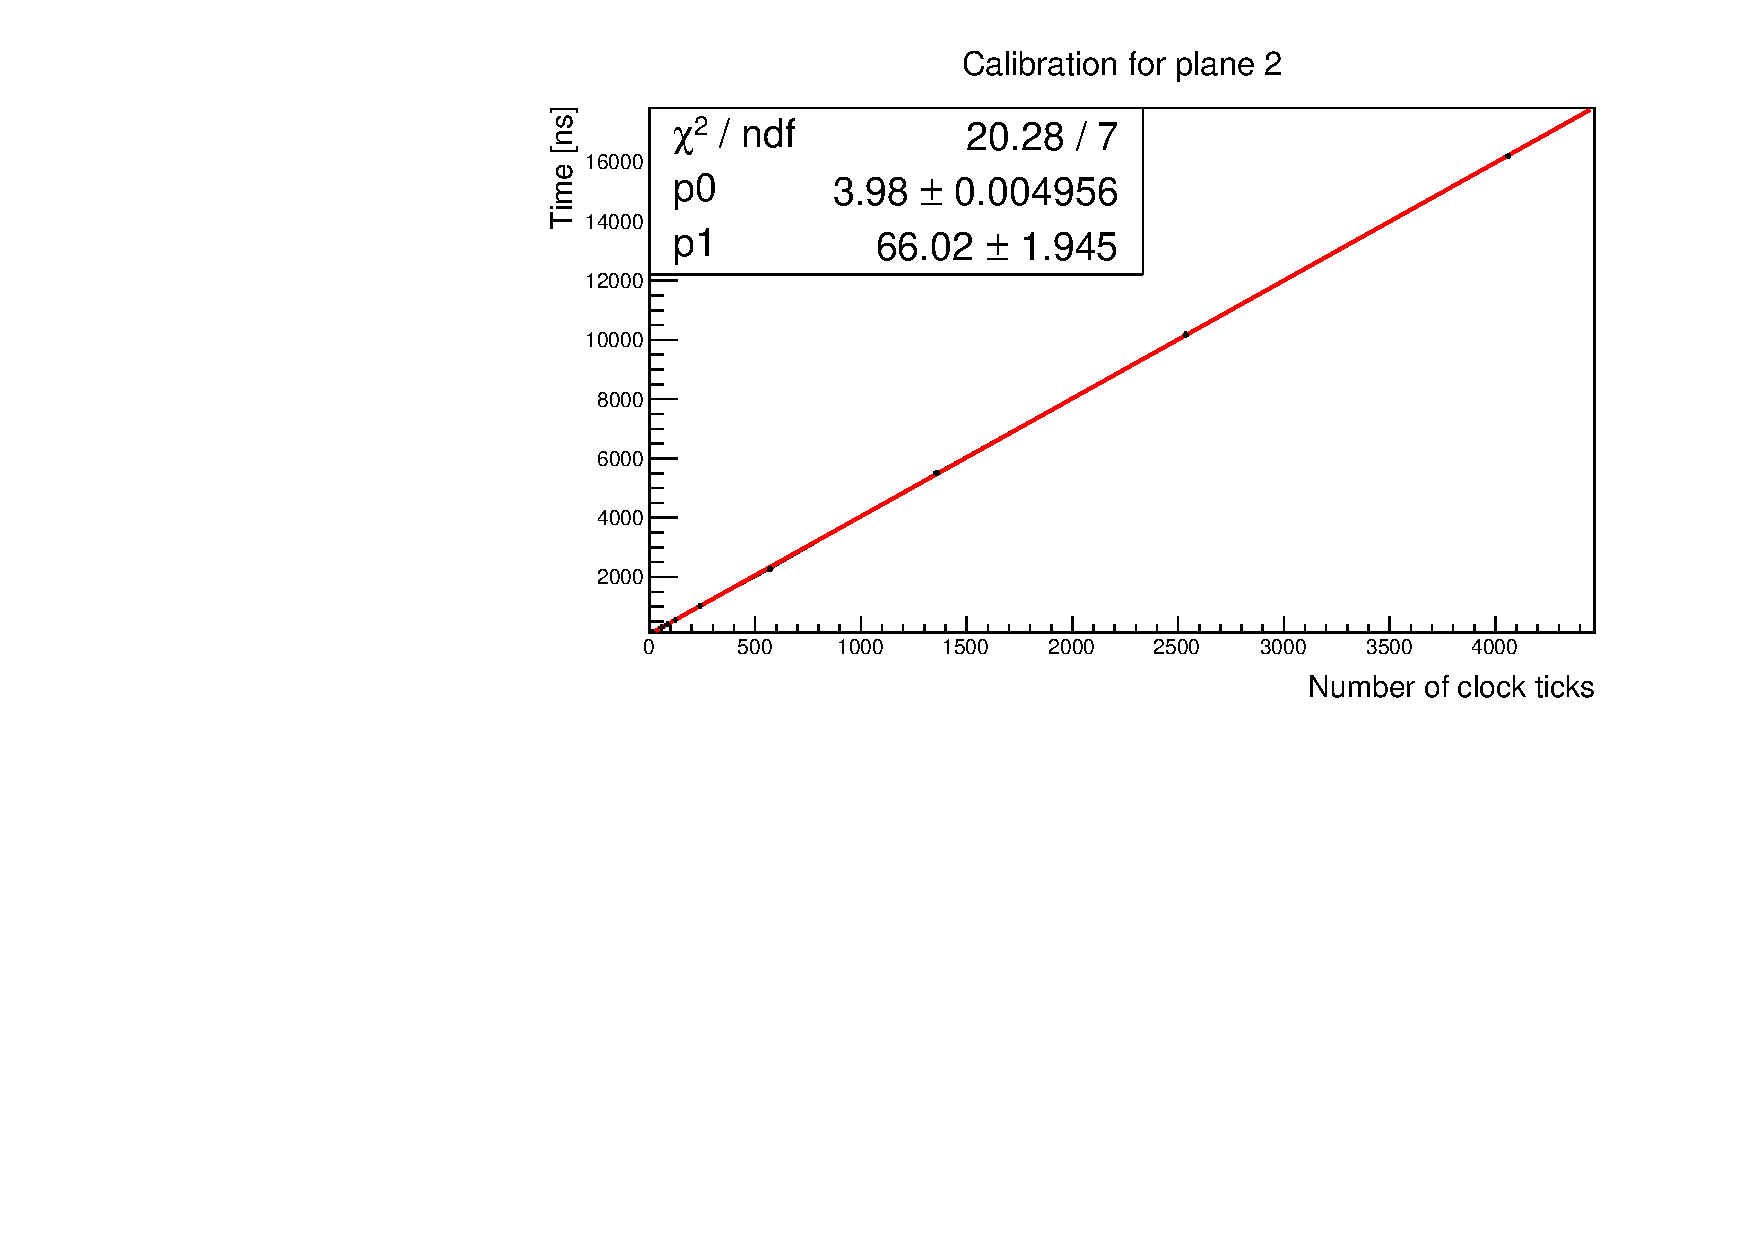
\includegraphics[width=0.7\linewidth]{images/calib_plane_2.pdf}}\\
 \subfloat[]{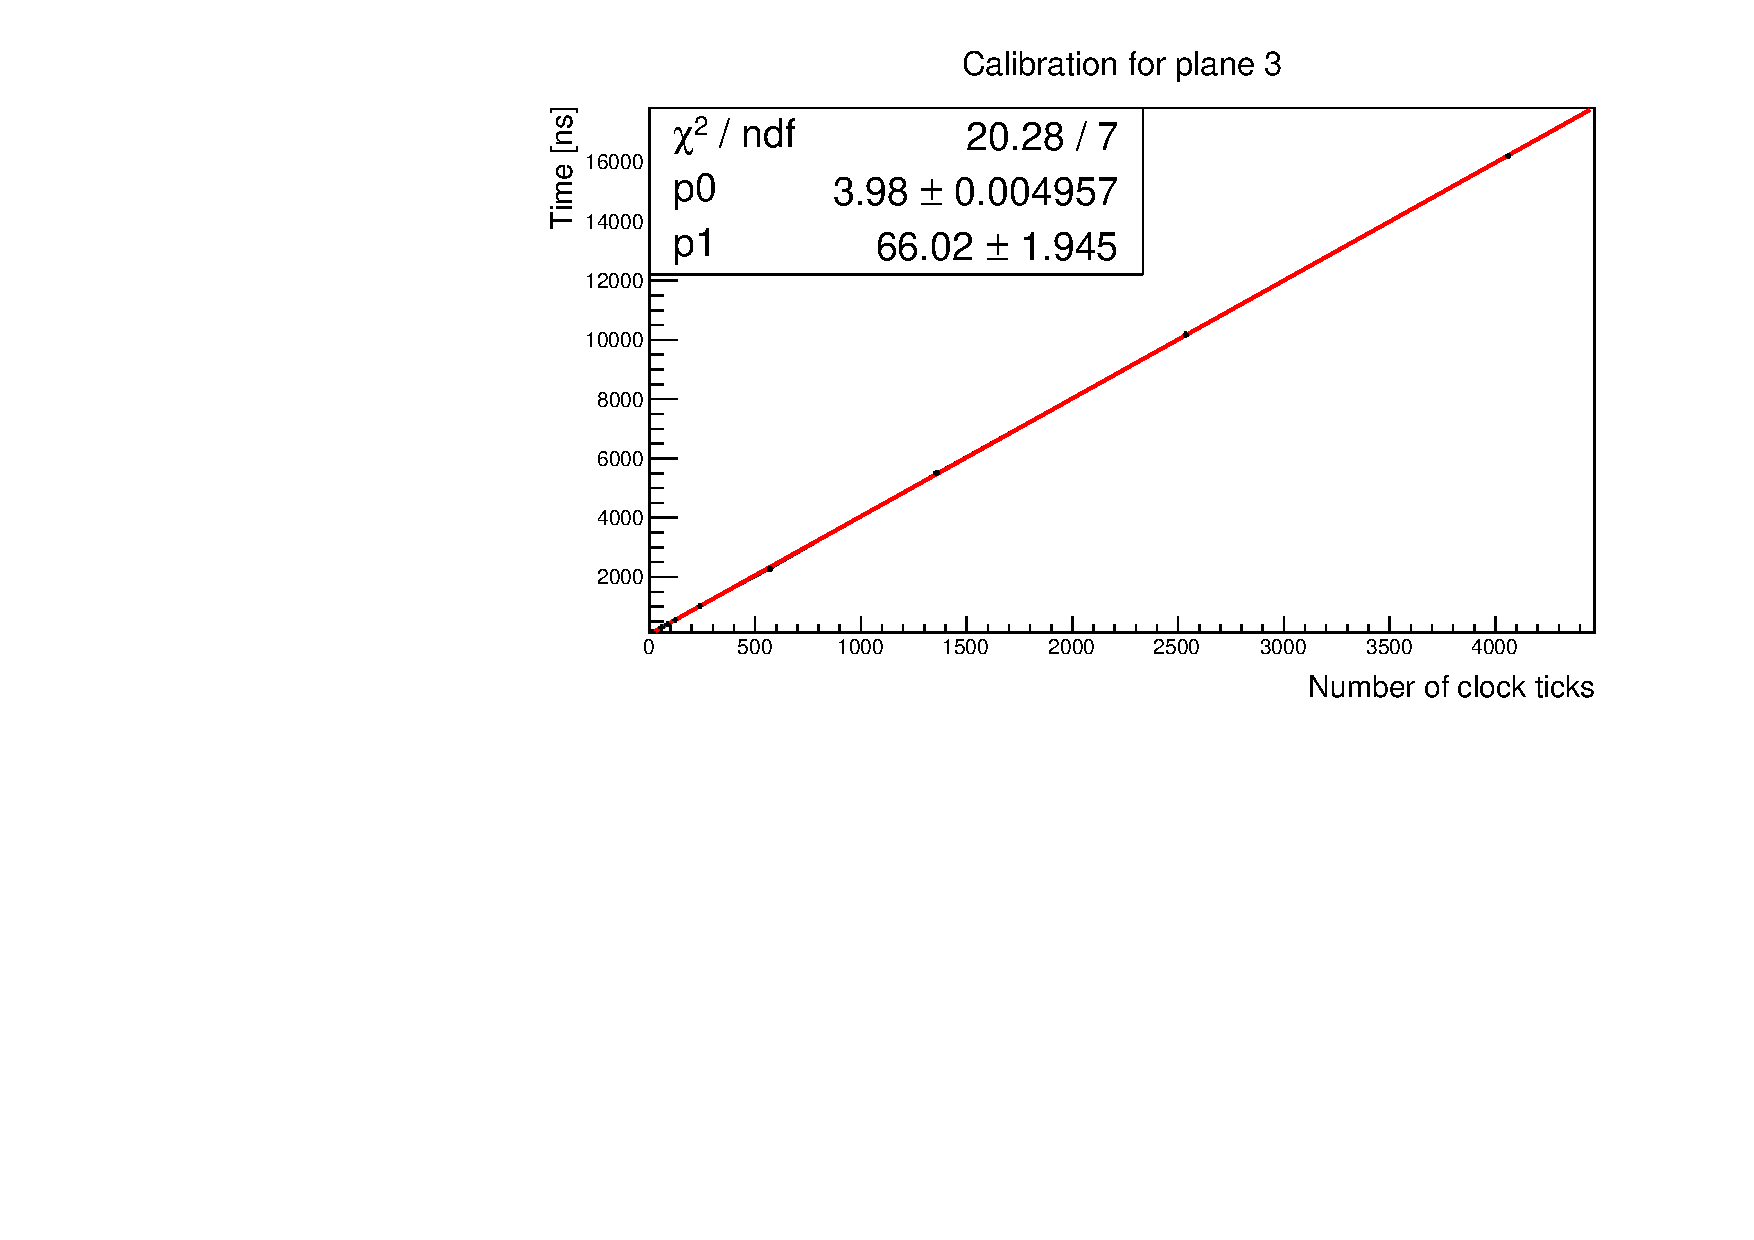
\includegraphics[width=0.7\linewidth]{images/calib_plane_3.pdf}}%
 \caption[Time calibration]{Time calibration for the different planes. In the fit p0 refers to the slope of the line and p1 to the y-intercept. All measures give a compatible clock-time conversion factor of \textnormal{3.98(0)}\,\si{\nano \second}\textnormal{/clock cycle}.}%
 \label{fig:timeCalibration}%
\end{figure}

\subsection{Signal Settings}
Another important step of the configuration is choosing the optimal signal width of the logic gates output. For example, the trigger implemented in the experiment, previously introduced in Subsection \ref{sub:detector}, works with a P1\,$\land$\,P2\,$\land$\,$\overline{\textnormal{P3}}$ logic, shown in Figure \ref{fig:TriggerLogic}. Clearly, if the P3 signal is not long enough it may lead to erroneous triggers as shown in Figure \ref{fig:wrongTrigger}. For this reason, the P3 signal has been chosen to be $\approx$80 ns wide,  while P1 and P2 were set at around $\approx$45 ns. Also small delays of $\approx$10 ns have been applied to P1 and P2 signals for the trigger to make sure they would be contained inside the full P3 veto signal, avoiding accidental triggering due to P1$\land$P2 being active before P3 activation.

\begin{figure}[hbt!]
   \centering
    

\tikzset{every picture/.style={line width=0.75pt}} %set default line width to 0.75pt        

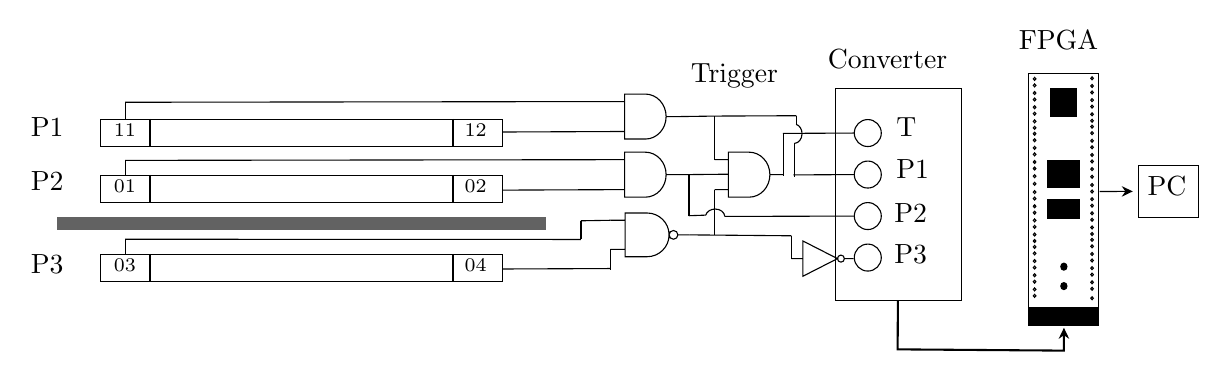
\begin{tikzpicture}[x=0.75pt,y=0.75pt,yscale=-1,xscale=1]
%uncomment if require: \path (0,300); %set diagram left start at 0, and has height of 300

%Shape: Rectangle [id:dp930181400844455] 
\draw   (75,59) -- (268.63,59) -- (268.63,71.99) -- (75,71.99) -- cycle ;
%Shape: Rectangle [id:dp08158386635903536] 
\draw   (75,85.99) -- (268.63,85.99) -- (268.63,98.97) -- (75,98.97) -- cycle ;
%Shape: Rectangle [id:dp24457282766289878] 
\draw  [draw opacity=0][fill={rgb, 255:red, 98; green, 98; blue, 98 }  ,fill opacity=1 ] (54,105.97) -- (289.63,105.97) -- (289.63,111.99) -- (54,111.99) -- cycle ;
%Shape: Rectangle [id:dp9901947676553108] 
\draw   (75,123.97) -- (268.63,123.97) -- (268.63,136.96) -- (75,136.96) -- cycle ;
%Shape: And Gate [id:dp6588905258750268] 
\draw   (327.33,46.72) -- (337.33,46.72) .. controls (342.85,46.72) and (347.33,51.58) .. (347.33,57.56) .. controls (347.33,63.53) and (342.85,68.39) .. (337.33,68.39) -- (327.33,68.39) -- (327.33,46.72) -- cycle (320.67,50.33) -- (327.33,50.33) (320.67,64.78) -- (327.33,64.78) (347.33,57.56) -- (354,57.56) ;
%Straight Lines [id:da6341381118531499] 
\draw    (98.67,58.67) -- (98.67,71.67) ;
%Straight Lines [id:da9227101082099702] 
\draw    (244.67,58.67) -- (244.67,71.67) ;
%Straight Lines [id:da4285928098073418] 
\draw    (244.67,85.67) -- (244.67,98.67) ;
%Straight Lines [id:da3413360036300346] 
\draw    (98.67,85.67) -- (98.67,98.67) ;
%Straight Lines [id:da5396247135072856] 
\draw    (244.67,123.67) -- (244.67,136.67) ;
%Straight Lines [id:da4982019005846289] 
\draw    (98.67,123.67) -- (98.67,136.67) ;
%Straight Lines [id:da7193934924500666] 
\draw    (86.67,50.67) -- (86.67,58.67) ;
%Straight Lines [id:da8043637118386225] 
\draw    (86.67,78.67) -- (86.67,85.67) ;
%Straight Lines [id:da7747602226999992] 
\draw    (86.67,116.67) -- (86.67,123.67) ;
%Straight Lines [id:da7833727015288415] 
\draw    (86.67,50.67) -- (320.67,50.33) ;
%Straight Lines [id:da9430802174606098] 
\draw    (86.67,78.67) -- (320.67,78.33) ;
%Straight Lines [id:da5632453946258708] 
\draw    (268.33,65) -- (320.67,64.78) ;
%Shape: And Gate [id:dp9933090209928017] 
\draw   (327.33,74.72) -- (337.33,74.72) .. controls (342.85,74.72) and (347.33,79.58) .. (347.33,85.56) .. controls (347.33,91.53) and (342.85,96.39) .. (337.33,96.39) -- (327.33,96.39) -- (327.33,74.72) -- cycle (320.67,78.33) -- (327.33,78.33) (320.67,92.78) -- (327.33,92.78) (347.33,85.56) -- (354,85.56) ;
%Straight Lines [id:da3911318303942659] 
\draw    (268.33,93) -- (320.67,92.78) ;
%Straight Lines [id:da16516466928273454] 
\draw    (86.67,116.67) -- (306.3,116.77) ;
%Straight Lines [id:da04392374129325016] 
\draw    (306.3,107.77) -- (306.3,116.77) ;
%Straight Lines [id:da20973150521783102] 
\draw    (306.3,107.77) -- (320.48,107.53) ;
%Straight Lines [id:da8921875351101065] 
\draw    (268.33,131) -- (320.67,130.78) ;
%Straight Lines [id:da3005758352671317] 
\draw    (320.67,121.44) -- (320.67,131.44) ;
%Shape: And Gate [id:dp7488715500500649] 
\draw   (377.33,74.72) -- (387.33,74.72) .. controls (392.85,74.72) and (397.33,79.58) .. (397.33,85.56) .. controls (397.33,91.53) and (392.85,96.39) .. (387.33,96.39) -- (377.33,96.39) -- (377.33,74.72) -- cycle (370.67,78.33) -- (377.33,78.33) (370.67,92.78) -- (377.33,92.78) (397.33,85.56) -- (404,85.56) ;
%Straight Lines [id:da10304511884327316] 
\draw    (370.67,57.33) -- (370.67,78.33) ;
%Straight Lines [id:da8662258575376999] 
\draw    (354,85.56) -- (377.33,85.33) ;
%Straight Lines [id:da745759473943691] 
\draw    (370.67,92.78) -- (370.67,114.78) ;
%Shape: Nand Gate [id:dp6457192512084823] 
\draw   (327.55,104.02) -- (338.16,104.02) .. controls (344.01,104.02) and (348.76,108.74) .. (348.76,114.56) .. controls (348.76,120.37) and (344.01,125.09) .. (338.16,125.09) -- (327.55,125.09) -- (327.55,104.02) -- cycle (320.48,107.53) -- (327.55,107.53) (320.48,121.58) -- (327.55,121.58) (353,114.56) -- (358.66,114.56) (348.76,114.56) .. controls (348.76,113.39) and (349.71,112.45) .. (350.88,112.45) .. controls (352.05,112.45) and (353,113.39) .. (353,114.56) .. controls (353,115.72) and (352.05,116.66) .. (350.88,116.66) .. controls (349.71,116.66) and (348.76,115.72) .. (348.76,114.56) -- cycle ;
%Straight Lines [id:da9181746311406199] 
\draw    (354,57.56) -- (370.67,57.33) ;
%Shape: Rectangle [id:dp6222782782547579] 
\draw   (429,44) -- (489.67,44) -- (489.67,146) -- (429,146) -- cycle ;
%Shape: Circle [id:dp004819883561298255] 
\draw   (438,65.5) .. controls (438,61.91) and (440.91,59) .. (444.5,59) .. controls (448.09,59) and (451,61.91) .. (451,65.5) .. controls (451,69.09) and (448.09,72) .. (444.5,72) .. controls (440.91,72) and (438,69.09) .. (438,65.5) -- cycle ;
%Shape: Circle [id:dp2273408824423182] 
\draw   (438,85.5) .. controls (438,81.91) and (440.91,79) .. (444.5,79) .. controls (448.09,79) and (451,81.91) .. (451,85.5) .. controls (451,89.09) and (448.09,92) .. (444.5,92) .. controls (440.91,92) and (438,89.09) .. (438,85.5) -- cycle ;
%Shape: Circle [id:dp3326276415223379] 
\draw   (438,105.5) .. controls (438,101.91) and (440.91,99) .. (444.5,99) .. controls (448.09,99) and (451,101.91) .. (451,105.5) .. controls (451,109.09) and (448.09,112) .. (444.5,112) .. controls (440.91,112) and (438,109.09) .. (438,105.5) -- cycle ;
%Shape: Circle [id:dp5894268738310305] 
\draw   (438,125.5) .. controls (438,121.91) and (440.91,119) .. (444.5,119) .. controls (448.09,119) and (451,121.91) .. (451,125.5) .. controls (451,129.09) and (448.09,132) .. (444.5,132) .. controls (440.91,132) and (438,129.09) .. (438,125.5) -- cycle ;
%Shape: Not/Inverter Gate [id:dp48109951495315173] 
\draw   (413.22,117.5) -- (429.89,126) -- (413.22,134.5) -- (413.22,117.5) -- cycle (407.67,126) -- (413.22,126) (433.22,126) -- (437.67,126) (429.89,126) .. controls (429.89,125.06) and (430.64,124.3) .. (431.56,124.3) .. controls (432.48,124.3) and (433.22,125.06) .. (433.22,126) .. controls (433.22,126.94) and (432.48,127.7) .. (431.56,127.7) .. controls (430.64,127.7) and (429.89,126.94) .. (429.89,126) -- cycle ;
%Straight Lines [id:da4272340949309752] 
\draw    (358.66,114.56) -- (407.67,115) ;
%Straight Lines [id:da6463698694739882] 
\draw    (407.67,115) -- (407.67,126) ;
%Straight Lines [id:da22464595123479336] 
\draw    (375.6,105.68) -- (438,105.5) ;
%Shape: Arc [id:dp9454271678978042] 
\draw  [draw opacity=0] (366.44,105.05) .. controls (366.88,103.37) and (368.74,102.11) .. (370.97,102.11) .. controls (373.47,102.11) and (375.51,103.7) .. (375.6,105.68) -- (370.97,105.82) -- cycle ; \draw   (366.44,105.05) .. controls (366.88,103.37) and (368.74,102.11) .. (370.97,102.11) .. controls (373.47,102.11) and (375.51,103.7) .. (375.6,105.68) ;  
%Straight Lines [id:da05133393965876054] 
\draw    (358.33,105.33) -- (366.44,105.05) ;
%Straight Lines [id:da03934384849007744] 
\draw    (358.33,85.33) -- (358.33,105.33) ;
%Straight Lines [id:da7513945899297801] 
\draw    (370.67,57.33) -- (410.07,57.15) ;
%Straight Lines [id:da5606323872818669] 
\draw    (404,86.06) -- (404,66.06) ;
%Shape: Rectangle [id:dp407309584327763] 
\draw   (522,37) -- (555.67,37) -- (555.67,158) -- (522,158) -- cycle ;
%Shape: Ellipse [id:dp31525641280410244] 
\draw   (524.24,39.41) .. controls (524.24,39.02) and (524.52,38.7) .. (524.87,38.7) .. controls (525.21,38.7) and (525.49,39.02) .. (525.49,39.41) .. controls (525.49,39.81) and (525.21,40.12) .. (524.87,40.12) .. controls (524.52,40.12) and (524.24,39.81) .. (524.24,39.41) -- cycle ;
%Shape: Ellipse [id:dp4738880085346945] 
\draw   (524.24,42.54) .. controls (524.24,42.15) and (524.52,41.83) .. (524.87,41.83) .. controls (525.21,41.83) and (525.49,42.15) .. (525.49,42.54) .. controls (525.49,42.93) and (525.21,43.25) .. (524.87,43.25) .. controls (524.52,43.25) and (524.24,42.93) .. (524.24,42.54) -- cycle ;
%Shape: Ellipse [id:dp6792192481762828] 
\draw   (524.24,46.23) .. controls (524.24,45.84) and (524.52,45.52) .. (524.87,45.52) .. controls (525.21,45.52) and (525.49,45.84) .. (525.49,46.23) .. controls (525.49,46.62) and (525.21,46.94) .. (524.87,46.94) .. controls (524.52,46.94) and (524.24,46.62) .. (524.24,46.23) -- cycle ;
%Shape: Ellipse [id:dp2765873209781733] 
\draw   (524.24,49.36) .. controls (524.24,48.96) and (524.52,48.65) .. (524.87,48.65) .. controls (525.21,48.65) and (525.49,48.96) .. (525.49,49.36) .. controls (525.49,49.75) and (525.21,50.07) .. (524.87,50.07) .. controls (524.52,50.07) and (524.24,49.75) .. (524.24,49.36) -- cycle ;
%Shape: Ellipse [id:dp24985562312808585] 
\draw   (524.24,53.05) .. controls (524.24,52.66) and (524.52,52.34) .. (524.87,52.34) .. controls (525.21,52.34) and (525.49,52.66) .. (525.49,53.05) .. controls (525.49,53.44) and (525.21,53.76) .. (524.87,53.76) .. controls (524.52,53.76) and (524.24,53.44) .. (524.24,53.05) -- cycle ;
%Shape: Ellipse [id:dp0881113365528503] 
\draw   (524.24,56.17) .. controls (524.24,55.78) and (524.52,55.46) .. (524.87,55.46) .. controls (525.21,55.46) and (525.49,55.78) .. (525.49,56.17) .. controls (525.49,56.56) and (525.21,56.88) .. (524.87,56.88) .. controls (524.52,56.88) and (524.24,56.56) .. (524.24,56.17) -- cycle ;
%Shape: Ellipse [id:dp7097000836768472] 
\draw   (524.24,59.87) .. controls (524.24,59.47) and (524.52,59.15) .. (524.87,59.15) .. controls (525.21,59.15) and (525.49,59.47) .. (525.49,59.87) .. controls (525.49,60.26) and (525.21,60.58) .. (524.87,60.58) .. controls (524.52,60.58) and (524.24,60.26) .. (524.24,59.87) -- cycle ;
%Shape: Ellipse [id:dp8266259432123018] 
\draw   (524.24,62.99) .. controls (524.24,62.6) and (524.52,62.28) .. (524.87,62.28) .. controls (525.21,62.28) and (525.49,62.6) .. (525.49,62.99) .. controls (525.49,63.38) and (525.21,63.7) .. (524.87,63.7) .. controls (524.52,63.7) and (524.24,63.38) .. (524.24,62.99) -- cycle ;
%Shape: Ellipse [id:dp4851938434830634] 
\draw   (524.24,65.83) .. controls (524.24,65.44) and (524.52,65.12) .. (524.87,65.12) .. controls (525.21,65.12) and (525.49,65.44) .. (525.49,65.83) .. controls (525.49,66.22) and (525.21,66.54) .. (524.87,66.54) .. controls (524.52,66.54) and (524.24,66.22) .. (524.24,65.83) -- cycle ;
%Shape: Ellipse [id:dp5674458649785409] 
\draw   (524.24,68.95) .. controls (524.24,68.56) and (524.52,68.24) .. (524.87,68.24) .. controls (525.21,68.24) and (525.49,68.56) .. (525.49,68.95) .. controls (525.49,69.35) and (525.21,69.66) .. (524.87,69.66) .. controls (524.52,69.66) and (524.24,69.35) .. (524.24,68.95) -- cycle ;
%Shape: Ellipse [id:dp1864083477977786] 
\draw   (524.24,72.65) .. controls (524.24,72.25) and (524.52,71.94) .. (524.87,71.94) .. controls (525.21,71.94) and (525.49,72.25) .. (525.49,72.65) .. controls (525.49,73.04) and (525.21,73.36) .. (524.87,73.36) .. controls (524.52,73.36) and (524.24,73.04) .. (524.24,72.65) -- cycle ;
%Shape: Ellipse [id:dp17394938634539447] 
\draw   (524.24,75.77) .. controls (524.24,75.38) and (524.52,75.06) .. (524.87,75.06) .. controls (525.21,75.06) and (525.49,75.38) .. (525.49,75.77) .. controls (525.49,76.16) and (525.21,76.48) .. (524.87,76.48) .. controls (524.52,76.48) and (524.24,76.16) .. (524.24,75.77) -- cycle ;
%Shape: Ellipse [id:dp46416853866560626] 
\draw   (524.24,79.46) .. controls (524.24,79.07) and (524.52,78.75) .. (524.87,78.75) .. controls (525.21,78.75) and (525.49,79.07) .. (525.49,79.46) .. controls (525.49,79.86) and (525.21,80.17) .. (524.87,80.17) .. controls (524.52,80.17) and (524.24,79.86) .. (524.24,79.46) -- cycle ;
%Shape: Ellipse [id:dp0930963445070273] 
\draw   (524.24,82.59) .. controls (524.24,82.2) and (524.52,81.88) .. (524.87,81.88) .. controls (525.21,81.88) and (525.49,82.2) .. (525.49,82.59) .. controls (525.49,82.98) and (525.21,83.3) .. (524.87,83.3) .. controls (524.52,83.3) and (524.24,82.98) .. (524.24,82.59) -- cycle ;
%Shape: Ellipse [id:dp48973686350608303] 
\draw   (524.24,86.28) .. controls (524.24,85.89) and (524.52,85.57) .. (524.87,85.57) .. controls (525.21,85.57) and (525.49,85.89) .. (525.49,86.28) .. controls (525.49,86.67) and (525.21,86.99) .. (524.87,86.99) .. controls (524.52,86.99) and (524.24,86.67) .. (524.24,86.28) -- cycle ;
%Shape: Ellipse [id:dp6775519722947608] 
\draw   (524.24,89.97) .. controls (524.24,89.58) and (524.52,89.26) .. (524.87,89.26) .. controls (525.21,89.26) and (525.49,89.58) .. (525.49,89.97) .. controls (525.49,90.37) and (525.21,90.68) .. (524.87,90.68) .. controls (524.52,90.68) and (524.24,90.37) .. (524.24,89.97) -- cycle ;
%Shape: Ellipse [id:dp7522526449700603] 
\draw   (524.24,93.95) .. controls (524.24,93.56) and (524.52,93.24) .. (524.87,93.24) .. controls (525.21,93.24) and (525.49,93.56) .. (525.49,93.95) .. controls (525.49,94.34) and (525.21,94.66) .. (524.87,94.66) .. controls (524.52,94.66) and (524.24,94.34) .. (524.24,93.95) -- cycle ;
%Shape: Ellipse [id:dp8007038633826975] 
\draw   (524.24,97.07) .. controls (524.24,96.68) and (524.52,96.36) .. (524.87,96.36) .. controls (525.21,96.36) and (525.49,96.68) .. (525.49,97.07) .. controls (525.49,97.47) and (525.21,97.78) .. (524.87,97.78) .. controls (524.52,97.78) and (524.24,97.47) .. (524.24,97.07) -- cycle ;
%Shape: Ellipse [id:dp5007466065606271] 
\draw   (524.24,100.77) .. controls (524.24,100.37) and (524.52,100.06) .. (524.87,100.06) .. controls (525.21,100.06) and (525.49,100.37) .. (525.49,100.77) .. controls (525.49,101.16) and (525.21,101.48) .. (524.87,101.48) .. controls (524.52,101.48) and (524.24,101.16) .. (524.24,100.77) -- cycle ;
%Shape: Ellipse [id:dp8643245281855352] 
\draw   (524.24,103.89) .. controls (524.24,103.5) and (524.52,103.18) .. (524.87,103.18) .. controls (525.21,103.18) and (525.49,103.5) .. (525.49,103.89) .. controls (525.49,104.28) and (525.21,104.6) .. (524.87,104.6) .. controls (524.52,104.6) and (524.24,104.28) .. (524.24,103.89) -- cycle ;
%Shape: Ellipse [id:dp9688781315769484] 
\draw   (524.24,107.58) .. controls (524.24,107.19) and (524.52,106.87) .. (524.87,106.87) .. controls (525.21,106.87) and (525.49,107.19) .. (525.49,107.58) .. controls (525.49,107.98) and (525.21,108.29) .. (524.87,108.29) .. controls (524.52,108.29) and (524.24,107.98) .. (524.24,107.58) -- cycle ;
%Shape: Ellipse [id:dp8981637163174572] 
\draw   (524.24,110.71) .. controls (524.24,110.32) and (524.52,110) .. (524.87,110) .. controls (525.21,110) and (525.49,110.32) .. (525.49,110.71) .. controls (525.49,111.1) and (525.21,111.42) .. (524.87,111.42) .. controls (524.52,111.42) and (524.24,111.1) .. (524.24,110.71) -- cycle ;
%Shape: Ellipse [id:dp16090338886523892] 
\draw   (524.24,114.4) .. controls (524.24,114.01) and (524.52,113.69) .. (524.87,113.69) .. controls (525.21,113.69) and (525.49,114.01) .. (525.49,114.4) .. controls (525.49,114.79) and (525.21,115.11) .. (524.87,115.11) .. controls (524.52,115.11) and (524.24,114.79) .. (524.24,114.4) -- cycle ;
%Shape: Ellipse [id:dp6316912579629486] 
\draw   (524.24,117.52) .. controls (524.24,117.13) and (524.52,116.81) .. (524.87,116.81) .. controls (525.21,116.81) and (525.49,117.13) .. (525.49,117.52) .. controls (525.49,117.92) and (525.21,118.23) .. (524.87,118.23) .. controls (524.52,118.23) and (524.24,117.92) .. (524.24,117.52) -- cycle ;
%Shape: Ellipse [id:dp9631005583187057] 
\draw   (524.24,120.37) .. controls (524.24,119.97) and (524.52,119.65) .. (524.87,119.65) .. controls (525.21,119.65) and (525.49,119.97) .. (525.49,120.37) .. controls (525.49,120.76) and (525.21,121.08) .. (524.87,121.08) .. controls (524.52,121.08) and (524.24,120.76) .. (524.24,120.37) -- cycle ;
%Shape: Ellipse [id:dp05264511791073179] 
\draw   (524.24,123.49) .. controls (524.24,123.1) and (524.52,122.78) .. (524.87,122.78) .. controls (525.21,122.78) and (525.49,123.1) .. (525.49,123.49) .. controls (525.49,123.88) and (525.21,124.2) .. (524.87,124.2) .. controls (524.52,124.2) and (524.24,123.88) .. (524.24,123.49) -- cycle ;
%Shape: Ellipse [id:dp2792412491912444] 
\draw   (524.24,127.18) .. controls (524.24,126.79) and (524.52,126.47) .. (524.87,126.47) .. controls (525.21,126.47) and (525.49,126.79) .. (525.49,127.18) .. controls (525.49,127.57) and (525.21,127.89) .. (524.87,127.89) .. controls (524.52,127.89) and (524.24,127.57) .. (524.24,127.18) -- cycle ;
%Shape: Ellipse [id:dp9826266351897567] 
\draw   (524.24,130.31) .. controls (524.24,129.91) and (524.52,129.6) .. (524.87,129.6) .. controls (525.21,129.6) and (525.49,129.91) .. (525.49,130.31) .. controls (525.49,130.7) and (525.21,131.02) .. (524.87,131.02) .. controls (524.52,131.02) and (524.24,130.7) .. (524.24,130.31) -- cycle ;
%Shape: Ellipse [id:dp30314368992174845] 
\draw   (524.24,134) .. controls (524.24,133.61) and (524.52,133.29) .. (524.87,133.29) .. controls (525.21,133.29) and (525.49,133.61) .. (525.49,134) .. controls (525.49,134.39) and (525.21,134.71) .. (524.87,134.71) .. controls (524.52,134.71) and (524.24,134.39) .. (524.24,134) -- cycle ;
%Shape: Ellipse [id:dp4775606847034566] 
\draw   (524.24,137.12) .. controls (524.24,136.73) and (524.52,136.41) .. (524.87,136.41) .. controls (525.21,136.41) and (525.49,136.73) .. (525.49,137.12) .. controls (525.49,137.52) and (525.21,137.83) .. (524.87,137.83) .. controls (524.52,137.83) and (524.24,137.52) .. (524.24,137.12) -- cycle ;
%Shape: Ellipse [id:dp7737621883340005] 
\draw   (524.24,140.82) .. controls (524.24,140.42) and (524.52,140.11) .. (524.87,140.11) .. controls (525.21,140.11) and (525.49,140.42) .. (525.49,140.82) .. controls (525.49,141.21) and (525.21,141.53) .. (524.87,141.53) .. controls (524.52,141.53) and (524.24,141.21) .. (524.24,140.82) -- cycle ;
%Shape: Ellipse [id:dp3136158433820917] 
\draw   (524.24,143.94) .. controls (524.24,143.55) and (524.52,143.23) .. (524.87,143.23) .. controls (525.21,143.23) and (525.49,143.55) .. (525.49,143.94) .. controls (525.49,144.33) and (525.21,144.65) .. (524.87,144.65) .. controls (524.52,144.65) and (524.24,144.33) .. (524.24,143.94) -- cycle ;
%Shape: Ellipse [id:dp9143532517986134] 
\draw   (551.93,39.13) .. controls (551.93,38.74) and (552.21,38.42) .. (552.55,38.42) .. controls (552.89,38.42) and (553.17,38.74) .. (553.17,39.13) .. controls (553.17,39.52) and (552.89,39.84) .. (552.55,39.84) .. controls (552.21,39.84) and (551.93,39.52) .. (551.93,39.13) -- cycle ;
%Shape: Ellipse [id:dp26362208348594585] 
\draw   (551.93,42.82) .. controls (551.93,42.43) and (552.21,42.11) .. (552.55,42.11) .. controls (552.89,42.11) and (553.17,42.43) .. (553.17,42.82) .. controls (553.17,43.21) and (552.89,43.53) .. (552.55,43.53) .. controls (552.21,43.53) and (551.93,43.21) .. (551.93,42.82) -- cycle ;
%Shape: Ellipse [id:dp35209922701887797] 
\draw   (551.93,45.95) .. controls (551.93,45.56) and (552.21,45.24) .. (552.55,45.24) .. controls (552.89,45.24) and (553.17,45.56) .. (553.17,45.95) .. controls (553.17,46.34) and (552.89,46.66) .. (552.55,46.66) .. controls (552.21,46.66) and (551.93,46.34) .. (551.93,45.95) -- cycle ;
%Shape: Ellipse [id:dp08865799237691385] 
\draw   (551.93,49.64) .. controls (551.93,49.25) and (552.21,48.93) .. (552.55,48.93) .. controls (552.89,48.93) and (553.17,49.25) .. (553.17,49.64) .. controls (553.17,50.03) and (552.89,50.35) .. (552.55,50.35) .. controls (552.21,50.35) and (551.93,50.03) .. (551.93,49.64) -- cycle ;
%Shape: Ellipse [id:dp6907301894956204] 
\draw   (551.93,52.76) .. controls (551.93,52.37) and (552.21,52.05) .. (552.55,52.05) .. controls (552.89,52.05) and (553.17,52.37) .. (553.17,52.76) .. controls (553.17,53.16) and (552.89,53.47) .. (552.55,53.47) .. controls (552.21,53.47) and (551.93,53.16) .. (551.93,52.76) -- cycle ;
%Shape: Ellipse [id:dp30540447501816204] 
\draw   (551.93,56.46) .. controls (551.93,56.06) and (552.21,55.75) .. (552.55,55.75) .. controls (552.89,55.75) and (553.17,56.06) .. (553.17,56.46) .. controls (553.17,56.85) and (552.89,57.17) .. (552.55,57.17) .. controls (552.21,57.17) and (551.93,56.85) .. (551.93,56.46) -- cycle ;
%Shape: Ellipse [id:dp9120396922053884] 
\draw   (551.93,59.58) .. controls (551.93,59.19) and (552.21,58.87) .. (552.55,58.87) .. controls (552.89,58.87) and (553.17,59.19) .. (553.17,59.58) .. controls (553.17,59.97) and (552.89,60.29) .. (552.55,60.29) .. controls (552.21,60.29) and (551.93,59.97) .. (551.93,59.58) -- cycle ;
%Shape: Ellipse [id:dp20505074595571604] 
\draw   (551.93,62.42) .. controls (551.93,62.03) and (552.21,61.71) .. (552.55,61.71) .. controls (552.89,61.71) and (553.17,62.03) .. (553.17,62.42) .. controls (553.17,62.81) and (552.89,63.13) .. (552.55,63.13) .. controls (552.21,63.13) and (551.93,62.81) .. (551.93,62.42) -- cycle ;
%Shape: Ellipse [id:dp7194165993691664] 
\draw   (551.93,65.55) .. controls (551.93,65.15) and (552.21,64.84) .. (552.55,64.84) .. controls (552.89,64.84) and (553.17,65.15) .. (553.17,65.55) .. controls (553.17,65.94) and (552.89,66.26) .. (552.55,66.26) .. controls (552.21,66.26) and (551.93,65.94) .. (551.93,65.55) -- cycle ;
%Shape: Ellipse [id:dp022826389177345474] 
\draw   (551.93,69.24) .. controls (551.93,68.85) and (552.21,68.53) .. (552.55,68.53) .. controls (552.89,68.53) and (553.17,68.85) .. (553.17,69.24) .. controls (553.17,69.63) and (552.89,69.95) .. (552.55,69.95) .. controls (552.21,69.95) and (551.93,69.63) .. (551.93,69.24) -- cycle ;
%Shape: Ellipse [id:dp2955394379634577] 
\draw   (551.93,72.36) .. controls (551.93,71.97) and (552.21,71.65) .. (552.55,71.65) .. controls (552.89,71.65) and (553.17,71.97) .. (553.17,72.36) .. controls (553.17,72.75) and (552.89,73.07) .. (552.55,73.07) .. controls (552.21,73.07) and (551.93,72.75) .. (551.93,72.36) -- cycle ;
%Shape: Ellipse [id:dp8907218027212775] 
\draw   (551.93,76.06) .. controls (551.93,75.66) and (552.21,75.35) .. (552.55,75.35) .. controls (552.89,75.35) and (553.17,75.66) .. (553.17,76.06) .. controls (553.17,76.45) and (552.89,76.77) .. (552.55,76.77) .. controls (552.21,76.77) and (551.93,76.45) .. (551.93,76.06) -- cycle ;
%Shape: Ellipse [id:dp12543186014133778] 
\draw   (551.93,79.18) .. controls (551.93,78.79) and (552.21,78.47) .. (552.55,78.47) .. controls (552.89,78.47) and (553.17,78.79) .. (553.17,79.18) .. controls (553.17,79.57) and (552.89,79.89) .. (552.55,79.89) .. controls (552.21,79.89) and (551.93,79.57) .. (551.93,79.18) -- cycle ;
%Shape: Ellipse [id:dp2777931718982476] 
\draw   (551.93,82.87) .. controls (551.93,82.48) and (552.21,82.16) .. (552.55,82.16) .. controls (552.89,82.16) and (553.17,82.48) .. (553.17,82.87) .. controls (553.17,83.26) and (552.89,83.58) .. (552.55,83.58) .. controls (552.21,83.58) and (551.93,83.26) .. (551.93,82.87) -- cycle ;
%Shape: Ellipse [id:dp43005947908434905] 
\draw   (551.93,86.56) .. controls (551.93,86.17) and (552.21,85.85) .. (552.55,85.85) .. controls (552.89,85.85) and (553.17,86.17) .. (553.17,86.56) .. controls (553.17,86.96) and (552.89,87.27) .. (552.55,87.27) .. controls (552.21,87.27) and (551.93,86.96) .. (551.93,86.56) -- cycle ;
%Shape: Ellipse [id:dp5578266916722441] 
\draw   (551.93,90.54) .. controls (551.93,90.15) and (552.21,89.83) .. (552.55,89.83) .. controls (552.89,89.83) and (553.17,90.15) .. (553.17,90.54) .. controls (553.17,90.93) and (552.89,91.25) .. (552.55,91.25) .. controls (552.21,91.25) and (551.93,90.93) .. (551.93,90.54) -- cycle ;
%Shape: Ellipse [id:dp6167241957946717] 
\draw   (551.93,93.67) .. controls (551.93,93.27) and (552.21,92.96) .. (552.55,92.96) .. controls (552.89,92.96) and (553.17,93.27) .. (553.17,93.67) .. controls (553.17,94.06) and (552.89,94.38) .. (552.55,94.38) .. controls (552.21,94.38) and (551.93,94.06) .. (551.93,93.67) -- cycle ;
%Shape: Ellipse [id:dp35712130643754214] 
\draw   (551.93,97.36) .. controls (551.93,96.97) and (552.21,96.65) .. (552.55,96.65) .. controls (552.89,96.65) and (553.17,96.97) .. (553.17,97.36) .. controls (553.17,97.75) and (552.89,98.07) .. (552.55,98.07) .. controls (552.21,98.07) and (551.93,97.75) .. (551.93,97.36) -- cycle ;
%Shape: Ellipse [id:dp25737724240336357] 
\draw   (551.93,100.48) .. controls (551.93,100.09) and (552.21,99.77) .. (552.55,99.77) .. controls (552.89,99.77) and (553.17,100.09) .. (553.17,100.48) .. controls (553.17,100.87) and (552.89,101.19) .. (552.55,101.19) .. controls (552.21,101.19) and (551.93,100.87) .. (551.93,100.48) -- cycle ;
%Shape: Ellipse [id:dp23701525147562552] 
\draw   (551.93,104.17) .. controls (551.93,103.78) and (552.21,103.46) .. (552.55,103.46) .. controls (552.89,103.46) and (553.17,103.78) .. (553.17,104.17) .. controls (553.17,104.57) and (552.89,104.88) .. (552.55,104.88) .. controls (552.21,104.88) and (551.93,104.57) .. (551.93,104.17) -- cycle ;
%Shape: Ellipse [id:dp6816135670772704] 
\draw   (551.93,107.3) .. controls (551.93,106.91) and (552.21,106.59) .. (552.55,106.59) .. controls (552.89,106.59) and (553.17,106.91) .. (553.17,107.3) .. controls (553.17,107.69) and (552.89,108.01) .. (552.55,108.01) .. controls (552.21,108.01) and (551.93,107.69) .. (551.93,107.3) -- cycle ;
%Shape: Ellipse [id:dp4133285407162661] 
\draw   (551.93,110.99) .. controls (551.93,110.6) and (552.21,110.28) .. (552.55,110.28) .. controls (552.89,110.28) and (553.17,110.6) .. (553.17,110.99) .. controls (553.17,111.38) and (552.89,111.7) .. (552.55,111.7) .. controls (552.21,111.7) and (551.93,111.38) .. (551.93,110.99) -- cycle ;
%Shape: Ellipse [id:dp650766540763064] 
\draw   (551.93,114.12) .. controls (551.93,113.72) and (552.21,113.41) .. (552.55,113.41) .. controls (552.89,113.41) and (553.17,113.72) .. (553.17,114.12) .. controls (553.17,114.51) and (552.89,114.83) .. (552.55,114.83) .. controls (552.21,114.83) and (551.93,114.51) .. (551.93,114.12) -- cycle ;
%Shape: Ellipse [id:dp2740432353445794] 
\draw   (551.93,116.96) .. controls (551.93,116.56) and (552.21,116.25) .. (552.55,116.25) .. controls (552.89,116.25) and (553.17,116.56) .. (553.17,116.96) .. controls (553.17,117.35) and (552.89,117.67) .. (552.55,117.67) .. controls (552.21,117.67) and (551.93,117.35) .. (551.93,116.96) -- cycle ;
%Shape: Ellipse [id:dp29211989003529815] 
\draw   (551.93,120.08) .. controls (551.93,119.69) and (552.21,119.37) .. (552.55,119.37) .. controls (552.89,119.37) and (553.17,119.69) .. (553.17,120.08) .. controls (553.17,120.47) and (552.89,120.79) .. (552.55,120.79) .. controls (552.21,120.79) and (551.93,120.47) .. (551.93,120.08) -- cycle ;
%Shape: Ellipse [id:dp30191975044221486] 
\draw   (551.93,123.77) .. controls (551.93,123.38) and (552.21,123.06) .. (552.55,123.06) .. controls (552.89,123.06) and (553.17,123.38) .. (553.17,123.77) .. controls (553.17,124.17) and (552.89,124.48) .. (552.55,124.48) .. controls (552.21,124.48) and (551.93,124.17) .. (551.93,123.77) -- cycle ;
%Shape: Ellipse [id:dp2594608512411257] 
\draw   (551.93,126.9) .. controls (551.93,126.51) and (552.21,126.19) .. (552.55,126.19) .. controls (552.89,126.19) and (553.17,126.51) .. (553.17,126.9) .. controls (553.17,127.29) and (552.89,127.61) .. (552.55,127.61) .. controls (552.21,127.61) and (551.93,127.29) .. (551.93,126.9) -- cycle ;
%Shape: Ellipse [id:dp3305004357671293] 
\draw   (551.93,130.59) .. controls (551.93,130.2) and (552.21,129.88) .. (552.55,129.88) .. controls (552.89,129.88) and (553.17,130.2) .. (553.17,130.59) .. controls (553.17,130.98) and (552.89,131.3) .. (552.55,131.3) .. controls (552.21,131.3) and (551.93,130.98) .. (551.93,130.59) -- cycle ;
%Shape: Ellipse [id:dp1158749199341641] 
\draw   (551.93,133.71) .. controls (551.93,133.32) and (552.21,133) .. (552.55,133) .. controls (552.89,133) and (553.17,133.32) .. (553.17,133.71) .. controls (553.17,134.11) and (552.89,134.42) .. (552.55,134.42) .. controls (552.21,134.42) and (551.93,134.11) .. (551.93,133.71) -- cycle ;
%Shape: Ellipse [id:dp17190557514417937] 
\draw   (551.93,137.41) .. controls (551.93,137.02) and (552.21,136.7) .. (552.55,136.7) .. controls (552.89,136.7) and (553.17,137.02) .. (553.17,137.41) .. controls (553.17,137.8) and (552.89,138.12) .. (552.55,138.12) .. controls (552.21,138.12) and (551.93,137.8) .. (551.93,137.41) -- cycle ;
%Shape: Ellipse [id:dp6475046283968432] 
\draw   (551.93,140.53) .. controls (551.93,140.14) and (552.21,139.82) .. (552.55,139.82) .. controls (552.89,139.82) and (553.17,140.14) .. (553.17,140.53) .. controls (553.17,140.92) and (552.89,141.24) .. (552.55,141.24) .. controls (552.21,141.24) and (551.93,140.92) .. (551.93,140.53) -- cycle ;
%Shape: Ellipse [id:dp029014311998703746] 
\draw   (551.93,145.08) .. controls (551.93,144.68) and (552.21,144.37) .. (552.55,144.37) .. controls (552.89,144.37) and (553.17,144.68) .. (553.17,145.08) .. controls (553.17,145.47) and (552.89,145.79) .. (552.55,145.79) .. controls (552.21,145.79) and (551.93,145.47) .. (551.93,145.08) -- cycle ;
%Shape: Rectangle [id:dp8827810421432076] 
\draw  [fill={rgb, 255:red, 0; green, 0; blue, 0 }  ,fill opacity=1 ] (532.47,43.9) -- (545.04,43.9) -- (545.04,57.53) -- (532.47,57.53) -- cycle ;
%Shape: Rectangle [id:dp6639714938312453] 
\draw  [fill={rgb, 255:red, 0; green, 0; blue, 0 }  ,fill opacity=1 ] (530.98,78.84) -- (546.24,78.84) -- (546.24,91.62) -- (530.98,91.62) -- cycle ;
%Shape: Rectangle [id:dp41365767884153437] 
\draw  [fill={rgb, 255:red, 0; green, 0; blue, 0 }  ,fill opacity=1 ] (530.98,97.58) -- (546.24,97.58) -- (546.24,106.87) -- (530.98,106.87) -- cycle ;
%Shape: Ellipse [id:dp1726969867497461] 
\draw  [fill={rgb, 255:red, 0; green, 0; blue, 0 }  ,fill opacity=1 ] (537.48,129.87) .. controls (537.48,128.93) and (538.15,128.18) .. (538.97,128.18) .. controls (539.79,128.18) and (540.45,128.93) .. (540.45,129.87) .. controls (540.45,130.8) and (539.79,131.56) .. (538.97,131.56) .. controls (538.15,131.56) and (537.48,130.8) .. (537.48,129.87) -- cycle ;
%Shape: Ellipse [id:dp07422106756414149] 
\draw  [fill={rgb, 255:red, 0; green, 0; blue, 0 }  ,fill opacity=1 ] (537.48,139.24) .. controls (537.48,138.31) and (538.15,137.55) .. (538.97,137.55) .. controls (539.79,137.55) and (540.45,138.31) .. (540.45,139.24) .. controls (540.45,140.17) and (539.79,140.93) .. (538.97,140.93) .. controls (538.15,140.93) and (537.48,140.17) .. (537.48,139.24) -- cycle ;
%Shape: Rectangle [id:dp4351164859307427] 
\draw  [fill={rgb, 255:red, 0; green, 0; blue, 0 }  ,fill opacity=1 ] (522,149.48) -- (555.67,149.48) -- (555.67,158) -- (522,158) -- cycle ;

%Straight Lines [id:da5011725884206888] 
\draw [line width=0.75]    (459,146.33) -- (458.88,169.72) -- (539,170.33) -- (539,162.33) ;
\draw [shift={(539,159.33)}, rotate = 90] [fill={rgb, 255:red, 0; green, 0; blue, 0 }  ][line width=0.08]  [draw opacity=0] (5.36,-2.57) -- (0,0) -- (5.36,2.57) -- (3.56,0) -- cycle    ;
%Straight Lines [id:da053013656754011595] 
\draw    (556.17,93.67) -- (569.17,93.62) ;
\draw [shift={(572.17,93.61)}, rotate = 179.8] [fill={rgb, 255:red, 0; green, 0; blue, 0 }  ][line width=0.08]  [draw opacity=0] (5.36,-2.57) -- (0,0) -- (5.36,2.57) -- (3.56,0) -- cycle    ;
%Straight Lines [id:da9931590601940409] 
\draw    (403.6,65.68) -- (438,65.5) ;
%Shape: Arc [id:dp09295143614537238] 
\draw  [draw opacity=0] (409.97,61.32) .. controls (411.64,61.8) and (412.86,63.68) .. (412.82,65.91) .. controls (412.77,68.41) and (411.15,70.42) .. (409.16,70.47) -- (409.11,65.84) -- cycle ; \draw   (409.97,61.32) .. controls (411.64,61.8) and (412.86,63.68) .. (412.82,65.91) .. controls (412.77,68.41) and (411.15,70.42) .. (409.16,70.47) ;  
%Straight Lines [id:da5135073169004833] 
\draw    (409.97,57.32) -- (409.97,61.32) ;
%Straight Lines [id:da5451321371988912] 
\draw    (409.16,86.47) -- (409.16,70.47) ;
%Straight Lines [id:da5151151421364558] 
\draw    (408.6,85.68) -- (438,85.5) ;

% Text Node
\draw (40,57) node [anchor=north west][inner sep=0.75pt]   [align=left] {P1};
% Text Node
\draw (40,83) node [anchor=north west][inner sep=0.75pt]   [align=left] {P2};
% Text Node
\draw (40,123) node [anchor=north west][inner sep=0.75pt]   [align=left] {P3};
% Text Node
\draw (358,31) node [anchor=north west][inner sep=0.75pt]   [align=left] {Trigger};
% Text Node
\draw (80,125) node [anchor=north west][inner sep=0.75pt]   [align=left] {\scriptsize 03};
% Text Node
\draw (249,125) node [anchor=north west][inner sep=0.75pt]   [align=left] {\scriptsize 04};
% Text Node
\draw (249,60) node [anchor=north west][inner sep=0.75pt]   [align=left] {\scriptsize 12};
% Text Node
\draw (80,60) node [anchor=north west][inner sep=0.75pt]   [align=left] {\scriptsize 11};
% Text Node
\draw (80,87) node [anchor=north west][inner sep=0.75pt]   [align=left] {\scriptsize 01};
% Text Node
\draw (249,87) node [anchor=north west][inner sep=0.75pt]   [align=left] {\scriptsize 02};
% Text Node
\draw (424,24) node [anchor=north west][inner sep=0.75pt]   [align=left] {Converter};
% Text Node
\draw (516,15) node [anchor=north west][inner sep=0.75pt]   [align=left] {FPGA};
% Text Node
\draw    (575,81) -- (604,81) -- (604,106) -- (575,106) -- cycle  ;
\draw (578,85) node [anchor=north west][inner sep=0.75pt]   [align=left] {PC};
% Text Node
\draw (457,57) node [anchor=north west][inner sep=0.75pt]   [align=left] {T};
% Text Node
\draw (457,77) node [anchor=north west][inner sep=0.75pt]   [align=left] {P1};
% Text Node
\draw (456,98) node [anchor=north west][inner sep=0.75pt]   [align=left] {P2};
% Text Node
\draw (456,118) node [anchor=north west][inner sep=0.75pt]   [align=left] {P3};


\end{tikzpicture}

    \caption{Logic circuit of the experimental setup. Both the trigger and the acquisition logic are displayed.}
    \label{fig:TriggerLogic}
\end{figure}

\begin{figure}[htb!]
    \centering
    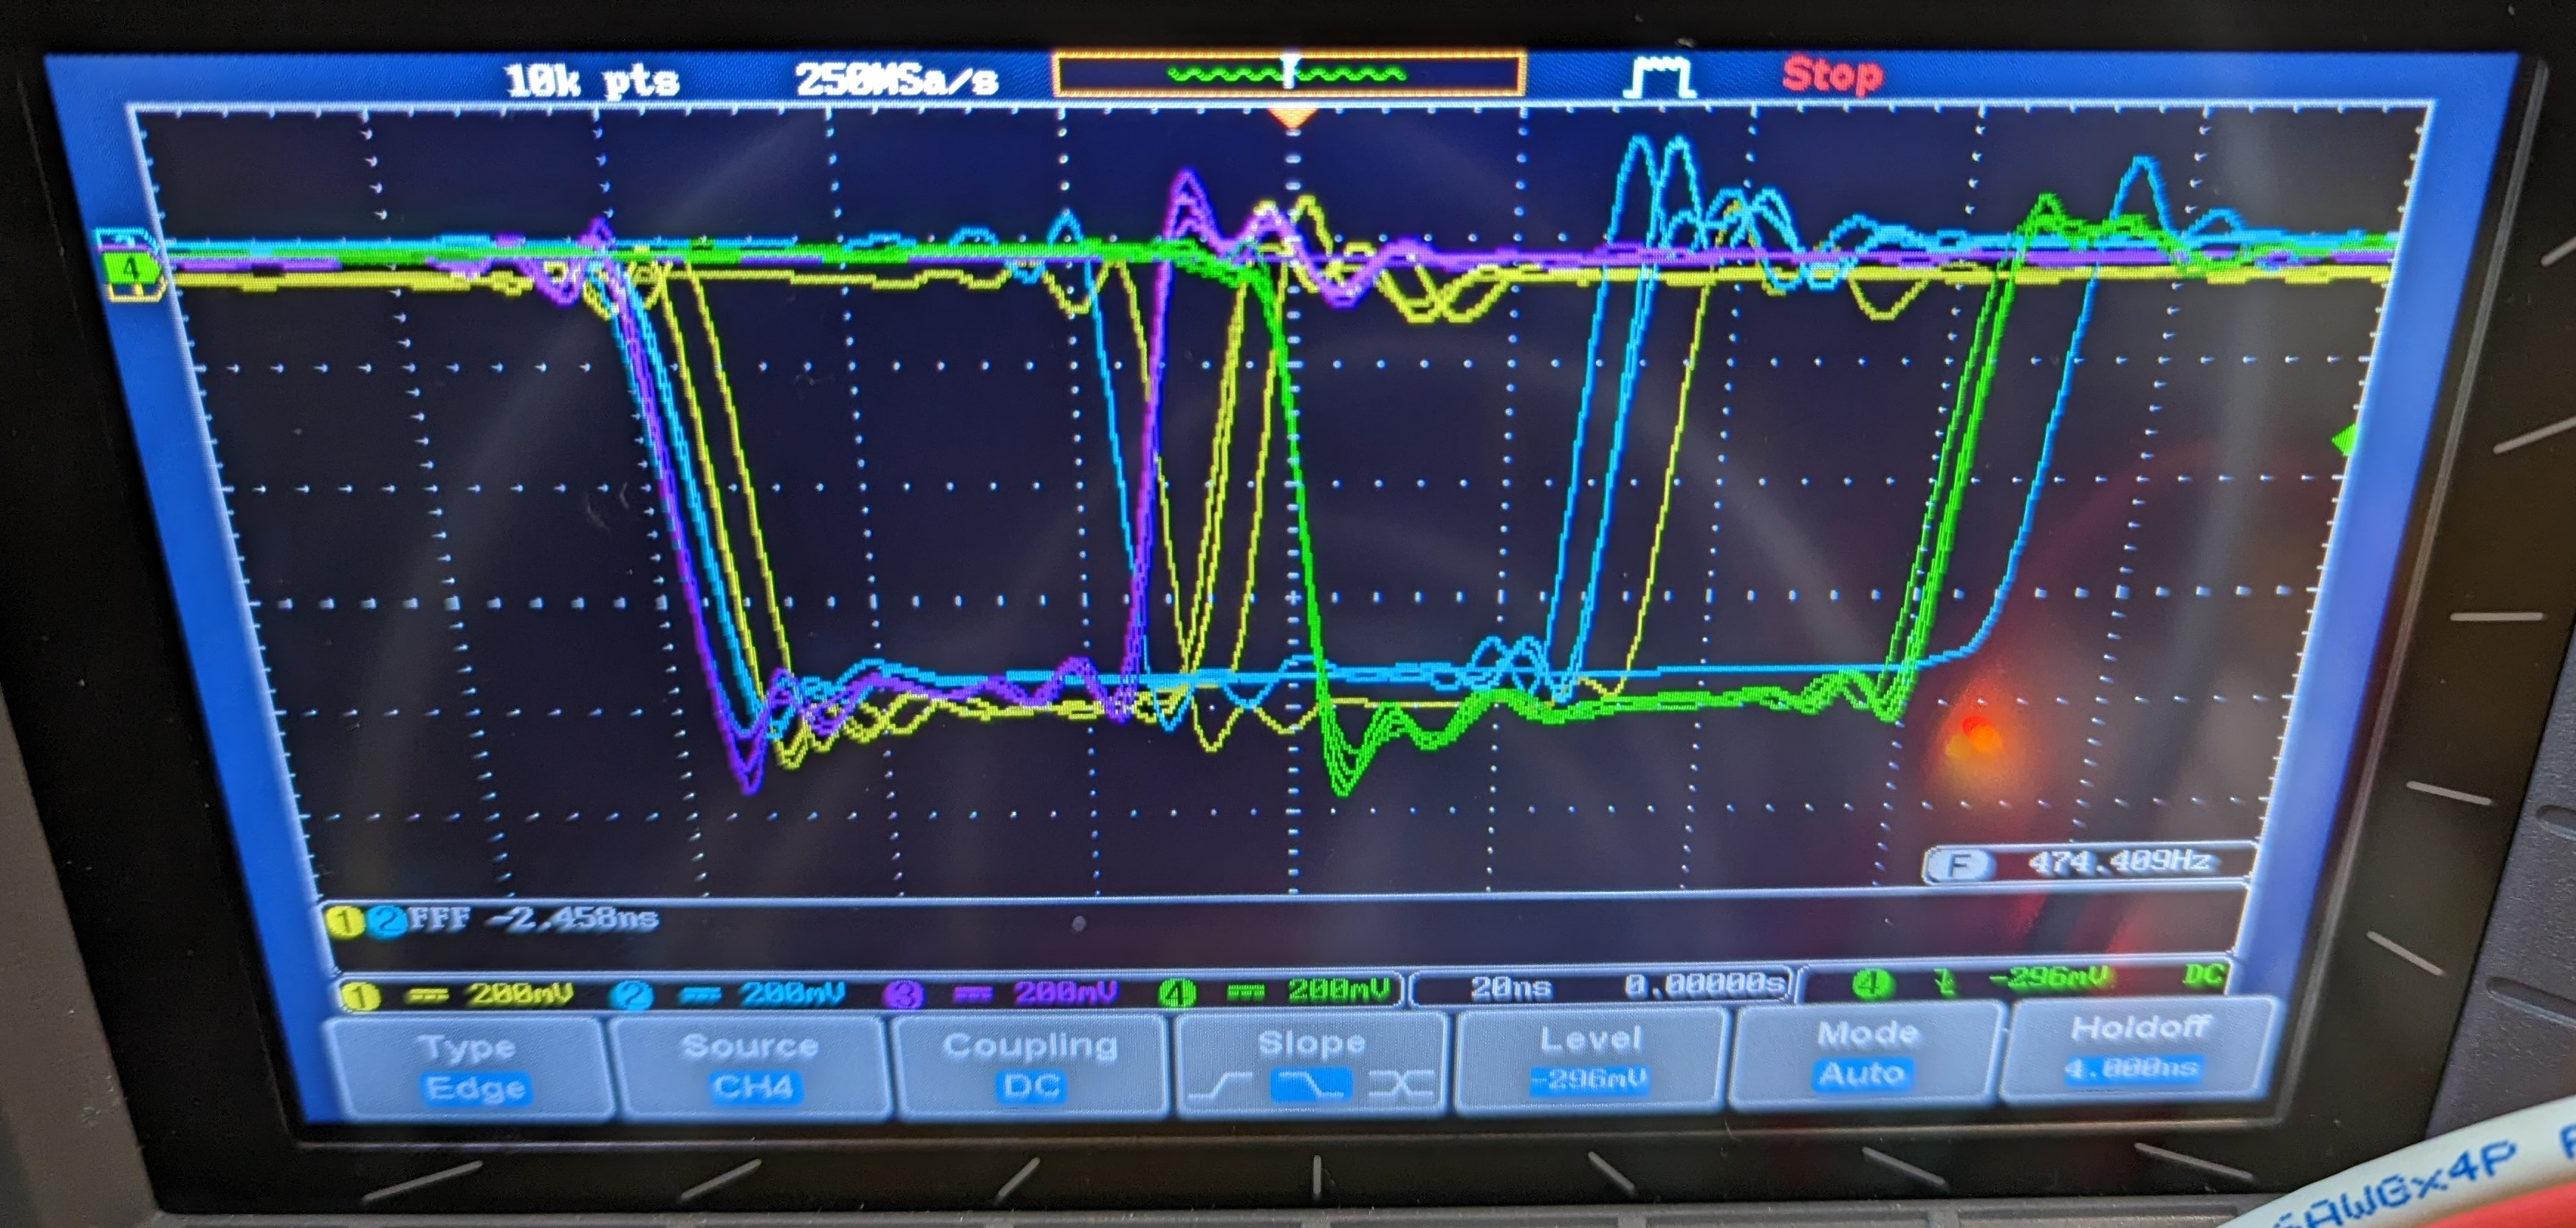
\includegraphics[width=0.8 \linewidth]{images/wrongtrigger.jpg}
    \caption{Trigger (4) activates because P3 (3) signal is not long enough to veto. Elongating P3 to switch on before and finish after P1 and P2 is an easy fix to make the system work correctly.}
    \label{fig:wrongTrigger}
\end{figure}

%\caption{Time calibration for the different planes.}
%\label{fig:timeCalibration}




\end{document}

\clearpage